\documentclass{article}
\usepackage{graphicx}


\PassOptionsToPackage{numbers}{natbib}


% ready for submission
\usepackage[final]{neurips_2023}

\usepackage{amsmath,amsfonts,amssymb,amsthm}

% to compile a preprint version, e.g., for submission to arXiv, add add the
% [preprint] option:
%     \usepackage[preprint]{neurips_2023}


% to compile a camera-ready version, add the [final] option, e.g.:
%     \usepackage[final]{neurips_2023}


% to avoid loading the natbib package, add option nonatbib:
%    \usepackage[nonatbib]{neurips_2023}


\usepackage[utf8]{inputenc} % allow utf-8 input
\usepackage[T1]{fontenc}    % use 8-bit T1 fonts
\usepackage[hidelinks]{hyperref}       % hyperlinks
\usepackage{url}            % simple URL typesetting
\usepackage{booktabs}       % professional-quality tables
\usepackage{nicefrac}       % compact symbols for 1/2, etc.
\usepackage{microtype}      % microtypography
\usepackage{xcolor}         % colors
\usepackage{cleveref}

\usepackage{graphicx}
\usepackage{caption}
\usepackage{subcaption}
\usepackage{float} % for H placement specifier

\newtheorem{theorem}{Theorem}[section]
\newtheorem{lemma}[theorem]{Lemma}
\newtheorem{proposition}[theorem]{Proposition}
\theoremstyle{definition}
\newtheorem{definition}[theorem]{Definition}
\newtheorem{example}[theorem]{Example}

\title{COMPSCI 683 Final Report}

\author{%
  Erin Song\\
  \texttt{esong@umass.edu} \\
  \And
  Harold Thidemann\\
  \texttt{hthidemann@umass.edu} \\
  \And
  Shubhang Vagvala\\
  \texttt{svagvala@umass.edu} \\
  \And
  Jiaqi Ye\\
  \texttt{jiaqiye@umass.edu} \\
}

\begin{document}

\maketitle
% \begin{abstract}
% Our project explores how to solve a Nurikabe puzzle of varying board sizes. The puzzle is a binary determination puzzle that is NP-complete, 
% meaning that the larger the board size, and exhaustive search would take a long time. We approach this problem as a Constraint Satisfaction 
% Problem (CSP) and use backtracking to solve it. There are also many prior inferences that can be made at the start of the puzzle. We find that --(insert relevant results and conclusions)--. 
% \end{abstract}

\section{Introduction}\label{sec:intro}
Our project explores how to solve Nurikabe, an island-forming puzzle. The puzzle is a binary determination puzzle that is NP-complete \cite{huttar}, meaning that the larger the board size, the longer time exhaustive search would take. We approach this problem as a Constraint Satisfaction Problem (CSP) and use backtracking to solve it. We implement some inferences that can be made at the start of the puzzle that can be found on \hyperlink{https://www.conceptispuzzles.com/index.aspx?uri=puzzle/nurikabe/techniques}{\underline{this website}} \cite{Inferences}. Figure 1 shows an example puzzle along with its solution. The rules can be found in the appendix (5.1). Our results show that our solver is accurate when solving boards but runs into speed issues on larger and more complex boards. 
% We denote each number and the respective white tiles around it, an "island." Islands must be isolated from each other which is done by adding black tiles. Nurikabe also has many starting inferences that can be made due to the location and size of islands. We implement a list of 18 inferences \cite{Inferences} that can be applied at the start of a game. These inferences are split into three sections: starting techniques [1.1 - 1.3], basic techniques [2.1 - 2.10], and advanced techniques [3.1 - 3.5]. 

\begin{figure}[h]
    \centering
    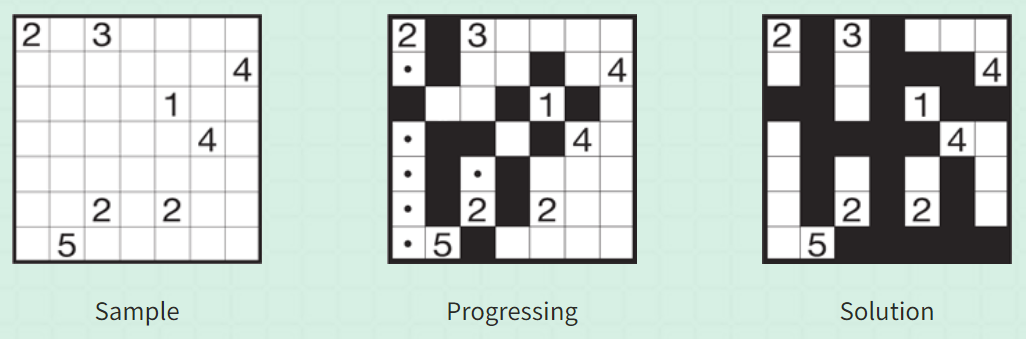
\includegraphics[width=0.6\textwidth]{example.png} \\
    \caption{A Nurikabe Puzzle and its Solution}
\end{figure}
\subsection{Our Contributions}\label{sec:contrib}
% We met weekly to discuss the work we've done the past week and our goals for next week.

\begin{enumerate}
    \item Erin Song: Wrote the intro and methodology for Inference, AC3, and difficulty metric. Wrote code for game constraints/rules and inferences [1.1, 2.1]. Designed equation for determining the difficulty of a puzzle.
    \item Harold Thidemann: Generated data set of boards. Wrote code for inferences [1.2, 1.3] and methods/graphs/difficulty code for testing the algorithm on various board sizes.
    \item Jiaqi Ye: Worked on code to generate data set of boards, reviewed related papers, developed basic backtracking algorithm for solving Nurikabe, wrote "Model and Preliminaries" and methodology for Backtracking.
    \item Shubhang Vagvala: Wrote code for inference [2.9], script to generate the test dataset and methods for testing the algorithm on various board sizes.
\end{enumerate}

\subsection{Related Work}\label{sec:related}

\hyperlink{https://theses.liacs.nl/pdf/18-JohanGroenen.pdf}{Johan Groenen} \cite{Groenen} explains how to solve all solvable puzzles and check for unique solvability using brute force algorithms, extended with backtracking and optimizations. The algorithm expands islands recursively, each time adding a cell from an island’s neighborhood to itself, and then updating the neighborhood. If the island is full, the next island is expanded. If there is no next island, we check if there are no pools and only one stream (which would make it a solution). You can reduce the search time by not allowing expansion to cells that have been tried earlier. We also looked at various other methods but did not use them. You can find a brief description of them in appendix 5.3.

\section{Model and Preliminaries}
Some of the notation below is based on the notation used in Groenen's \cite{Groenen} paper.

\subsection{Nurikabe Board, Islands, and Neighborhoods}
An $m \times n$ Nurikabe Board is a set of cells $C$ arranged in a grid with $m$ rows and $n$ columns. A \textit{seed cell} contains a number denoting the number of cells in its island. For a cell $a$, $v(a)$ is its assigned value.

We define an island to be its seed cell and the white cells in a connected mass containing the seed cell.

Two cells $x=(i_1, j_1)$ and $y=(i_2, j_2)$ are adjacent, indicated by $adj(x, y)$, if $|i_1-i_2|+|j_1-j_2|=1$. We define $neighborhood(I)$ of an island $I$ to be the set of cells adjacent to any cell $b$ in the island:
$neighborhood(I)= \{ a \in C | adj(a, b) \}$.

\subsection{Nurikabe Puzzle and Correct Solution}
We define a Nurikabe Puzzle to be a Nurikabe Board such that $\forall a\in C : v(a) \in \{ empty \} \cup Z^{+}$. 

A Correct Solution is a Nurikabe Board that meets all the constraints of the puzzle according to the rules (listed in appendix 5.1).

\subsection{Difficulty Calculations}
We define three criteria to determine a puzzle's difficulty which are board size, number of islands, and uniqueness of island seeds. We mathematically assign values less than 1 to all three and add them together and label those with sums in the range [0, 1] to be easy, [1, 2] to be medium, and [2, 3] to be hard. 
\begin{itemize}
\itemsep0em 
    \item $B_{m \times n}$: A board $B$ of dimensions $m\times n$ 
    \item $B_{area}$: Number of tiles in $B_{m \times n}$
    \item $total_w$: Sum of the island values in $B_{m\times n}$ which will be the final number of white tiles in a valid solution
    \item $total_b$: Total number of black tiles in $B_{m\times n}$ for a valid solution, this can be calculated without having the answer by doing $B_{area} - total_w$
    \item $I_{total}$: Total island seed cells on $B_{m \times n}$
    \item $I_{unique}$: Unique island seed cell values on $B_{m \times n}$
\end{itemize}
Using these definitions, we construct these functions
\begin{equation}
    f(B) = \frac{B_{m \times n}}{150} ,~~
    g(I) = \frac{I_{unique}}{I_{total}}  ,~~
    h(B) = 1 - \frac{|total_w - total_b|}{B_{area}}
\end{equation}
$f(B)$ calculates the ratio of the board to our largest test board of size 150 which gives us a numeric value that defines difficulty added by board size. $g(I)$ calculates the ratio of unique island seed cells to total number of island seed cells which gives us a numeric value that defines difficulty added by unique values. We only add $g(I)$ if $\frac{|total_w - total_b|}{B_{area}}$ is less than $\frac{1}{3}$ to account for a low $I_{total}$. In $h(B)$, we calculate $|total_w - total_b|$, because the smaller their difference, the less trivial a problem. A large amount of white tiles would mean a large island, a large amount of black tiles would mean many small islands, which we have determined are simple puzzles. We then need to divide by the area and subtract from 1 to ensure that this value is between [0, 1]. We want all 3 functions to be within this range so that the difficulty lies in the given ranges for easy, medium, and hard.

% \begin{equation}
%     \frac{B_{m \times n}}{150} + X + \left(1 - \frac{total_w - total_b}{B_{area}}\right) \mbox{~where~} X = 
%     \left\{ \begin{array}{rcl} 
%         \frac{I_{unique}}{I_{total}} & \mbox{if} & y    \\
%         0 & \mbox{if} & \neg y
%     \end{array} \right.
% \end{equation}

\section{Methodology}

% from jjay's report section draft
% There are many strategies that can be used to solve a given Nurikabe Puzzle P. If P has a  solution, we want to solve it and return the Correct Solution C for P. Taking inspiration from Johan Groenen’s backtracking strategy, we decided to solve the CSP using backtracking with pre-inferencing steps.
The following explains the main ideas used to solve a Nurikabe Puzzle. 

\subsection{Inference}
There are a list of inferences that can be made before backtracking \cite{Inferences}. We implement the starting technique inferences and some basic techniques before backtracking and call this pre-inferencing. Inferences for Nurikabe involve searching nearby tiles to determine if a tile should be black or white; however, due to the nature of our backtracking algorithm and constraint checking, we can only apply the inferences before backtracking. This is because our backtracking algorithm returns boards with default black tiles instead of default white tiles and the constraints are based off of the whole board state. This is a mistake in our design as we should have implemented the inferences before designing the backtracking and constraint checks. 

\subsection{Arc-Consistency}
AC3 can be applied to any CSP problem. We attempted implementing this throughout the backtracking; however, we realized that arc-consistency for Nurikabe would require island-specific constraints rather than the whole board evaluation since the "arcs" would be between islands. Our constraints check to see if a board state is solved or not, but does not check for if an individual island is within the rules. This was an overlook on our part and thus, we were unable to combine our arc-consistency code with the backtracking algorithm. 

\subsection{Backtracking}
% We chose to use a backtracking algorithm (Figure 4) because we defined the problem as a CSP, where each variables is an island $I$ to-be-expanded and domains are cells in $neighborhood(I)$. An island is selected for expansion using the most constrained variable criteria, which is having the least number of white cells further needed to complete the island because this is the island that is the most constrained, in the sense that it has the least number of expansions left to make. Ties are broken arbitrarily because we found that because there are so many different configurations of the board, it is difficult to know how a certain change would end up constraining the domains of other islands in the future.

% After selecting an island $I$, we order the cells in $neighborhood(I)$ using the least constraining value criteria, which is by shortest euclidean distance from the seed cell. We chose this method because, intuitively, adding cells closer to the center of the island keeps the island more condensed so that there is less chance of extending too far and 1) breaking the stream of black tiles, 2) getting too close to another island such that it severely constrains the other island’s domain.

% We deviate from the pseudocode (appendix 5.2) because we do not perform inferencing here, as explained in section 3.1

% Given more time, we would try to make a version that does inferencing while backtracking is still running. Some other possible extensions include finding a better way to break ties, accounting for possible duplicate states being checked while backtracking, and implementing reinforcement learning strategies.
We chose to use a modified backtracking algorithm (Figure 4) since the problem is a CSP and order of variable assignment is irrelevant. Each variable is an island $I$ to-be-expanded and domains are cells in $neighborhood(I)$. An island is selected for expansion using the most constrained variable criteria, which we define as having the least number of white cells further needed to complete the island because the domain is limited to fewer possible cell candidates for expansion. Ties are broken arbitrarily because we found that since there are so many configurations of the board, it is difficult to know how a certain change would end up constraining the domains of other islands in the future. After selecting an island $I$, we order the cells in $neighborhood(I)$ using the least constraining value criteria, which is by shortest euclidean distance from the seed cell. We chose this method because, intuitively, adding cells closer to the center of the island keeps islands more condensed so that there is less chance of extending too far and 1) breaking the stream of black tiles or 2) getting too close to another island such that it severely restricts the other island’s domain. We deviate from the pseudocode (appendix 5.2) because we do not perform inferencing here, as explained in section 3.1.

Given more time, we would try to make a version that does inferencing while backtracking is still running. Some other possible extensions include finding a better way to break ties, accounting for possible duplicate states being checked while backtracking, and implementing reinforcement learning strategies.

\subsection{Difficulty Rating}
One important metric when solving problems is to be able to solve both easy and hard problems. We determined three factors that contribute to the difficulty of a problem: board size, number of islands, and uniqueness of island seed cells. A larger board size generally means a more complex puzzle as there is a larger search space. Too many islands will simplify the puzzle as the numbers will all be small and too few would just mean a very large island. Thus, harder puzzles will be somewhere in between. Finally, the uniqueness of island seed cells can affect the difficulty. Take, for example, a board with only 1's. This puzzle will be very easy to solve. However, a board with [1,5,7,9,20,21] would be far more difficult to solve. See equation (1) for a detailed calculation.


\section{Results}

For our testing, we used a Nurikabe generator found on GitHub \cite{Malorn} to create a large dataset of boards. We limited the board size to test any board that has less than 150 cells. We also implemented a timeout function so if the solving of the board was taking too long, we would move on to the next board to test. This was done to ensure we were able to test in a reasonable time frame. These restrictions still allowed us to test $\approx 4800$ different boards (see Figure 2).

\begin{figure}[H]
    \begin{minipage}{.49\textwidth}
        \centering
        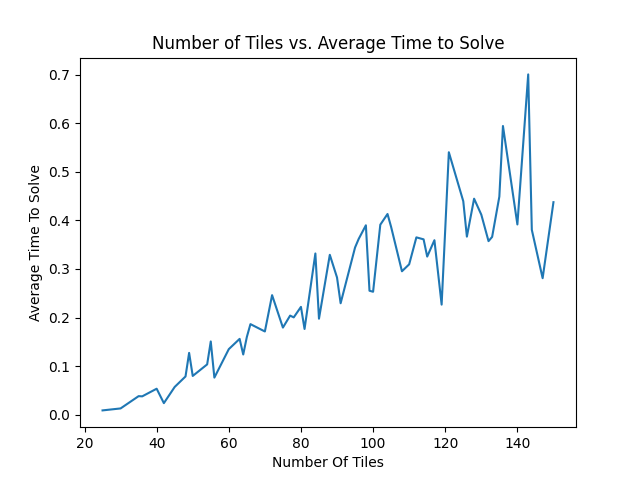
\includegraphics[width=1\linewidth]{num_tiles_vs_avg_solve_time.png}
    \end{minipage}
    \begin{minipage}{.49\textwidth}
        \centering
        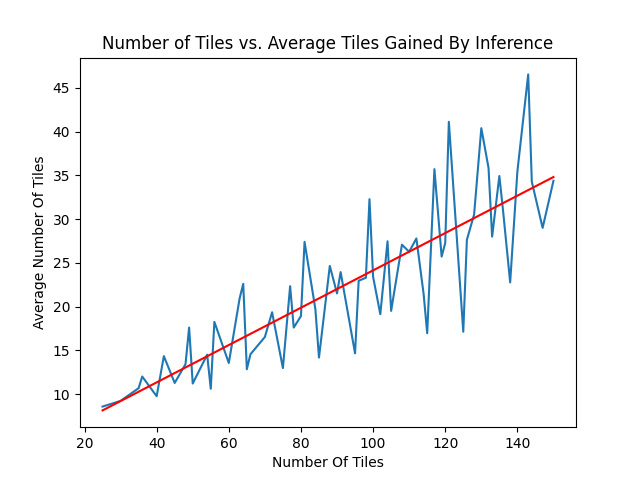
\includegraphics[width=1\linewidth]{num_tiles_vs_avg_tiles_from_inference.png}
    \end{minipage}
    \caption{The figure on the left shows the average time to solve vs the number of tiles in a board; The figure on the right shows average number of tiles gained by inference for a given board size, with a line of best fit.}
\end{figure}
The graph on the left in Figure 2 shows a positive correlation between the number of tiles on a board and the time to solve that given board size. This is expected as backtracking is a recursive function and larger boards have more potential board states that need to be explored. We hypothesize that given more inference methods the average time to solve a given board size would go down because the search space would decrease.

The graph on the right in Figure 2 shows a positive correlation between the number of tiles on the board and the average number of tiles gained by inference. The red line on the graph is the line of best fit, giving us our function for the number of tiles found by inference based on the number of tiles on the board. We observe that as the board sizes increase we find more tiles from inference, giving us confidence that our inference functions work well. If we had implemented more inferences we believe that the actual line of best fit would be close to a one to one function (number of tiles in the board is how many we get from inference).

\begin{figure}[H]
\begin{minipage}{0.49\textwidth}
    \centering
    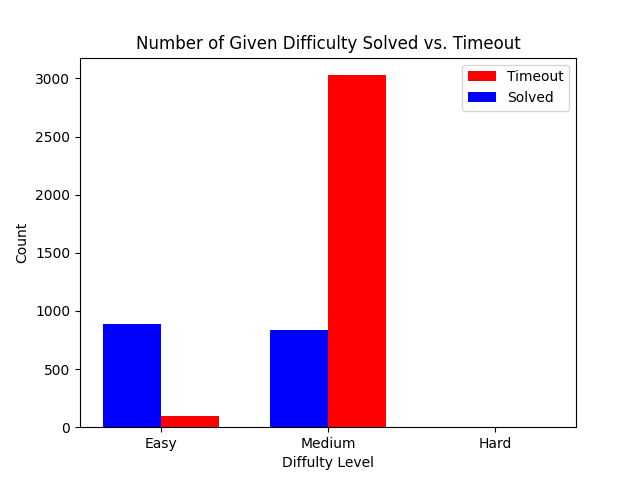
\includegraphics[width=1\linewidth]{num_of_difficulty_solved.png}
\end{minipage}
\begin{minipage}{0.49\textwidth}
    \centering
    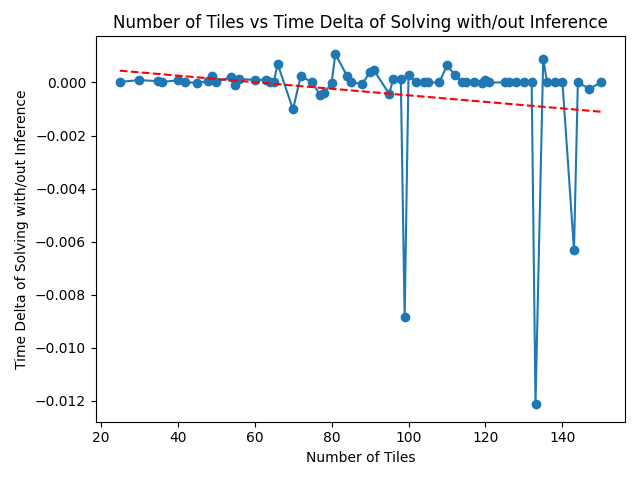
\includegraphics[width=1\linewidth]{num_tiles_vs_delta.png}
\end{minipage}
\caption{The graph on the left shows the count of how many boards were solved and how many hit the timeout limit for the given categories of difficulties. Note \textit{hard} has a count of 3 timeouts and none solved. The graph on the right shows the average time difference when solving the puzzles with and without using inferences versus the number of tiles in a board. }
\end{figure}
The results from the graph on the left follow from the previous results. It should be noted for this graph, the timeouts were set for 1 second. From the previous graphs we saw a positive correlation with the time to solve and the board size; this reinforces that idea. Larger boards are classified as harder compared to a smaller board. The effects of higher-complexity boards show in this graph as more of the medium-difficulty boards timed out as compared to the easy boards. 
These results may indicate that given more time, our solver would be able to solve larger (and harder) boards.


The trend from the graph on the right shows that for small boards, solving without inference is generally faster, while for medium-sized boards, the solving times are nearly equal with the odd deltas. However, as the board size increases further, solving using inference starts to outperform the without-inference approach slightly, and in some cases, by a significant margin. This observation aligns with intuition, as inference techniques have minimal impact on the state of small boards. However, as the board size grows, the effects of inference become more pronounced.


Please see section 5.5 in the appendix for the Github repository link.

\bibliographystyle{plain}
\bibliography{references}
% \appendix
\section{Appendix}

% You may include an appendix of arbitrary size to your submission. This may contain extra figures, experiments, discusion etc. Please do not assume that the course staff will read the appendix in detail. Your submission needs to be standalone.

\subsection{Nurikabe Rules and Background:}
Nurikabe puzzles were developed in Japan and published in a logic puzzle magazine from Nikoli in 1991. The puzzle consists of a grid board where each cell can have one of three states. Each cell can be either black, white or contain a number. The rules are as follows: 
\begin{enumerate}
    \item You cannot fill in cells containing numbers.
    \item A number tells the number of continuous white cells. Each area of white cells contains only one number in it and they are separated by black cells.
    \item The black cells are linked to be a continuous wall.
    \item Black cells cannot be linked to be 2×2 square or larger (sometimes referred to as a "pool")
\end{enumerate}


\subsection{Backtracking Pseudo-code}
\begin{figure}[H]
    \centering
    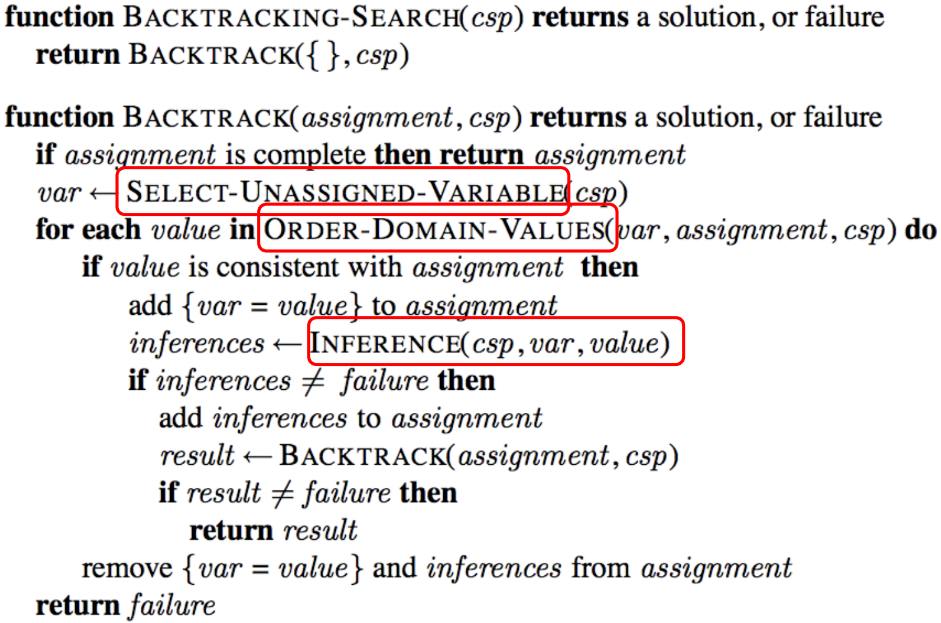
\includegraphics[width=0.7\textwidth]{backtracking.png} \\
    \caption{Backtracking Algorithm Pseudocode}
\end{figure}

\subsection{More Related Work}
\hyperlink{http://www.spenceryoungcs.com/nurikabeGA.html}{Spencer Young et al.} \cite{Young} developed a genetic algorithm solver for Nurikabe which can solve 5x5 Nurikabe problems in approx. 1 second. The solver uses all the traditional properties of genetic algorithms, such as population, mating pool, elitism, mutation, and breeding.

\hyperlink{https://dl.acm.org/doi/10.1145/3319619.3338470}{Martyn Amos et al.} \cite{Amos} made a Nurikabe solver using Ant Colony Optimization. 

\hyperlink{https://dl.acm.org/doi/pdf/10.5555/3447286.3447294}{Paul Bass et al.} \cite{Bass} took a scattered neighborly approach to solving Nurikabe. The method combines scatter search and variable neighorhood search. 

Nurikabe puzzles may also be encoded as SAT problems. \hyperlink{https://github.com/Microsoft/nurikabe}{Stephan T. Lavavej} \cite{Lavavej} developed an algorithm that solves Nurikabe using a SAT solver.

\subsection{Fun Graph}
\begin{figure}[H]
    \centering
    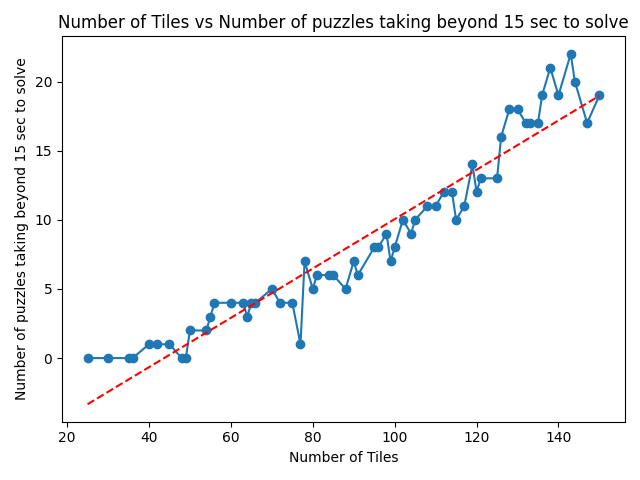
\includegraphics[width=0.7\linewidth]{num_tiles_vs_timeouts.png}
    \caption{This figure shows the number of puzzles taking longer than 15 seconds to solve versus the number of tiles in a board. This took a while to run (6 hours).}
\end{figure}
The graph shows a strong positive correlation between the number of tiles and the number of puzzles taking more than 15 seconds to solve. This clear trend indicates that larger puzzle boards directly result in a higher proportion of puzzles requiring extended solving time, demonstrating the increasing complexity and difficulty associated with solving puzzles as the board size grows.

\subsection{Github Repository}
Link to our repository:
\hyperlink{https://github.com/harhacking/683-Nurikabe}{https://github.com/harhacking/683-Nurikabe}

The repository is currently private as such that link won't work. Please email hthideman@umass.edu for access and it will be granted if requested. Note that the code within the repository is the same code that was submitted.

\end{document}